\documentclass[10pt,a4paper]{article}
\usepackage[utf8]{inputenc}
\usepackage[catalan]{babel}
\usepackage{multicol}
\usepackage{graphicx}
\usepackage{fancyhdr}
\usepackage{times}
\usepackage{titlesec}
\usepackage{multirow}
\usepackage{lettrine}
\usepackage[top=2cm, bottom=1.5cm, left=2cm, right=2cm]{geometry}
\usepackage[figurename=Fig.,tablename=TAULA]{caption}
\usepackage{hyperref}
\usepackage[ampersand]{easylist}
\usepackage{listings}
\usepackage[dvipsnames]{xcolor}

\lstset{
  breaklines=true,
  tabsize=2,
}

\captionsetup[table]{textfont=sc}

\titlespacing*{\section}{0pt}{0.5cm}{0.2cm}
\titlespacing*{\subsection}{0pt}{0.5cm}{0.2cm}


\graphicspath{{img/}}

\author{\normalsize\sffamily Kevin Martín Fernández}
\title{\huge{\sffamily Informe de seguiment I}}
\date{}

\newcommand\blfootnote[1]{%
  \begingroup
  \renewcommand\thefootnote{}\footnote{#1}%
  \addtocounter{footnote}{-1}%
  \endgroup
}

%No ident
\setlength\parindent{0pt}

%
%\large\bfseries\sffamily
\titleformat{\section}
{\large\sffamily\scshape\bfseries}
{\textbf{\thesection}}{1em}{}

\begin{document}

\fancyhead[LO]{\scriptsize Kevin Martín: Entorn de simulació per la captura d'imatges des de dron}
\fancyhead[RO]{\thepage}
\fancyhead[LE]{\thepage}
\fancyhead[RE]{\scriptsize EE/UAB TFG INFORMÀTICA: Entorn de simulació per la captura d'imatges des de dron}

\fancyfoot[CO,CE]{}

\fancypagestyle{primerapagina}
{
   \fancyhf{}
   \fancyhead[L]{\scriptsize TFG EN ENGINYERIA INFORMÀTICA, ESCOLA D'ENGINYERIA (EE), UNIVERSITAT AUTÒNOMA DE BARCELONA (UAB)}
   \fancyfoot[C]{\scriptsize Abril de 2019, Escola d'Enginyeria (UAB)}
}

%\lhead{\thepage}
%\chead{}
%\rhead{\tiny EE/UAB TFG INFORMÀTICA: TÍTOL (ABREUJAT SI ÉS MOLT LLARG)}
%\lhead{ EE/UAB \thepage}
%\lfoot{}
%\cfoot{\tiny{February 2015, Escola d'Enginyeria (UAB)}}
%\rfoot{}
\renewcommand{\headrulewidth}{0pt}
\renewcommand{\footrulewidth}{0pt}
\pagestyle{fancy}

%\thispagestyle{myheadings}

\maketitle

\thispagestyle{primerapagina}
%\twocolumn[\begin{@twocolumnfalse}
%\maketitle
%\begin{abstract}
\begin{center}
\parbox{0.915\textwidth}

\bigskip

{\vrule depth 0pt height 0.5pt width 4cm\hspace{7.5pt}%
\raisebox{-3.5pt}{\fontfamily{pzd}\fontencoding{U}\fontseries{m}\fontshape{n}\fontsize{11}{12}\selectfont\char70}%
\hspace{7.5pt}\vrule depth 0pt height 0.5pt width 4cm\relax}

\end{center}

\bigskip
%\end{abstract}

\vspace{-1cm}

\section{Actualització dels objectius}
En aquest apartat veurem els objectius complets (Verd) i els objectius que estan començats però no acabats (Taronja).

\begin{easylist}
\ListProperties(Progressive*=0.5cm)
& \textcolor{ForestGreen}{Analitzar}

& Definir
&& \textcolor{ForestGreen}{Definir mòduls interessants pel projecte}
&& \textcolor{ForestGreen}{Definir l'estructura del software}
&& Definir plataformes utilitzades 
&&& \textcolor{ForestGreen}{Definir els mòduls a desenvolupar}
&&& \textcolor{ForestGreen}{Definir la comunicació entre els mòduls}
&&& \textcolor{RedOrange}{Definir estructura de les dades que rebrà Unreal Engine}

& Desenvolupar
&& \textcolor{ForestGreen}{Desenvolupar mòdul de transformació i obtenció de dades}
&& Desenvolupar mòdul gràfic (Ureal Engine)
&&& Desenvolupar la interfície del menú
&&& \textcolor{RedOrange}{Desenvolupar la lògica del vehicle}
&&& Desenvolupar codi per la carrega de terreny y material
&&& \textcolor{RedOrange}{Desenvolupar llibreria RPC per el control del entorn}

&& Desenvolupar mòdul de scripting
&&& Desenvolupament client que controlarà el vehicle
&& Integrar els mòduls d'AirSim en Unreal Engine
&&& Integrar mòdul de Segmentació en el projecte
&& Desenvolupar altres capes d'informació

& Testejar
&& Fer provés del mòdul de transformació de dades
&& \textcolor{RedOrange}{Fer provés del mòdul gràfic}
&& Fer provés del mòdul de control per scripting
&&& Elaborar script d'exemple
&&& Provar script d'exemple

& Documentar
&& \textcolor{ForestGreen}{Redactar informe inicial}
&& \textcolor{ForestGreen}{Redactar informe de seguiment I}
&& Redactar informe de seguiment II
&& Redactar l'informe final
&& Elaborar proposta de presentació
&& Elaborar pòster
&& \textcolor{RedOrange}{Gestionar la documentació del dossier}
\end{easylist}


\section{Mòdul GeoTools}

Mòdul generat en Python amb l'objectiu d'obtenir informació de mapes d'elevacions, ortofotos, etc. Amb l'objectiu posterior de fer un tractament d'aquestes dades per la generació de terrenys tridimensional i informació en format visible per tal de poder visualitzar-ho en un motor gràfic de tipus Unreal, Unity, OpenGL, etc.

\subsection{Obtenció de dades}

Amb l'objectiu d'obtenir dades geogràfiques s'ha optat per la comunicació amb els estàndards proposats per l'Open Geospatial Consortium\cite{ogc}: Web Map Service\cite{wms} encarregat de posar a disponibilitat dades d'imatge com poden ser ortofotos d'una zona geogràfica seleccionada i Web Coverage Service\cite{wcs} encarregat de retornar informació referent a les elevacions de terreny en una zona geogràfica concreta. Per tal d'obtenir dades es fan peticions HTTP a les direccions web oferides per distintes institucions que segueixen els estàndard anomenats, en aquest cas s'ha realitzat proves amb l'Institut Cartogràfic i Geològic de Catalunya\cite{icgc}.

\subsubsection{Fitxer de configuració}

Per tal de determinar quines dades volem obtenir i de quins webservices l'aplicació accepta per paràmetre un fitxer de configuració en format JSON que ens permet determinar diferents propietats de les dades que demanarem com es pot veure en l'apèndix \ref{appendix:geotoolconfig}. En aquest fitxer es pot configurar els següents paràmetres:

\begin{easylist}[itemize]
& \textbf{Type}: Fa referència al tipus de coordenades que li passarem, pot ser latlong o xy en el primer cas farà la corresponent transformació al format UTM (xy)
& \textbf{Coordinates}: Coordenades sobre les quals volem fer la petició en el format indicat en el camp type. Si s'escull "xy" es definirà els atributs x, y en cas d'escollir "latlong" definirem els atributs lat, long.
& \textbf{Dimensions}: En aquesta secció escollirem les dimensions que volem que es demanin en les peticions per tal de mantenir la mateixa zona geogràfica.
&& Bbox: Aquestes seran les dimensions de la zona que volem obtenir amb les que es calcularà els límits que delimitaran la zona.
&& Texture: Aquesta serà la resolució que obtindrem per les diferents textures.
& \textbf{Wcsurl}: URL al webservice que ens donarà les dades d'altures.
& \textbf{Outputwcs}: Nom de sortida del fitxer generat per les altures
& \textbf{Formatwcs}: Format del fitxer generat per les altures. Disponibles: raw, obj (Objecte 3D)
& \textbf{Wmsrequests}: Array amb cada una de les peticions que farem a diferents WMS per tal d'obtenir vàries imatges
&& Url: URL al webservice WMS
&& Layers: capa o capes que volem obtenir d'aquests webservice
&& Output: Nom del fitxer de sortida
&& OutputFormat: Format del fitxer de sortida. Disponibles: JPG
\end{easylist}

\subsection{Generació de Terrenys a partir dun mapa d'altures}
En aquesta secció s'explicarà les diverses formes que s'han optat per generar terrenys que puguin ser interpretats en diferents motors gràfics.

\subsubsection{Format RAW}
El format RAW és un format pla que es basa en guarda en valors de 16 Bytes totes les altures en format binari tenim com a referència del mar el valor 128, i afegits en el fitxer un darrere de l'altre. Aquest format és acceptat per al creador de terrenys d'Unreal i Unity, però té certes limitacions de dimensions que s'han de complir especificades a l'editor en crear el terreny que fa que es perdi el control de la malla generada, les coordenades de textura no coincideixen amb la textura que es vol aplicar al terreny. Motius pels quals s'ha optat per afegir la generació de l'objecte 3D en format estàndard definit nosaltres l'objecte com es podrà veure en l'apartat \ref{mesh3d}, ja que aquestes limitacions fan que es facin vàries adaptacions no estàndards perquè es pugui visualitzar correctament.

\subsubsection{Generació de malla 3D}
\label{mesh3d}
Per tal d'importar terrenys en els motors gràfics s'ha optat per generar una malla 3D en format Wavefront obj\cite{wavefrontobj} format compatible amb qualsevol editor 3D, motor gràfic, etc. Aquest format dóna la llibertat per tal de controla la distància entre els vèrtexs, on s'aplicarà la textura i quines seran les normals dels vèrtexs fent que el terreny sigui suavitzat.
\\
\\
Com que el tractament amb bucles és lent s'ha realitzat tots els càlculs amb la llibreria NumPy aprofitant l'eficiència que incorpora aquesta llibreria amb el càlcul de matrius pel qual s'ha adaptat el problema com podem veure en el codi disponible en l'annex \ref{appendix:generateobj}.
\\
\\
Per la generació d'objectes cal definir 4 tipus d'objectes:

\begin{easylist}
& \textbf{Vèrtex}: Són cada un dels punts en el món, van definits pels índexs segons llegui'm la graella d'elevacions, es multipliquen per un K (Distancia entre els vèrtexs segons la distància que ens indiqui el mapa d'elevacions obtingut).

& \textbf{Vèrtex de textura}: Vèrtex amb dos components x, y compresos entre el 0 i 1 que indican la correspondència entre els punts d'una textura i la malla en la qual es vol aplicar aquella textura. Aquestes propietats es calcularien amb les equacions \ref{equation:u} i \ref{equation:v}.
\begin{equation}
\label{equation:u}
u = f(columna) = columna / (ample - 1)
\end{equation}
\begin{equation}
\label{equation:v}
v = f(fila) = 1 - (fila / (altura - 1))
\end{equation}

& \textbf{Normal del vèrtex}: Vectors que ens indica la direcció en la qual es reflecteix la llum per a cada vèrtex de l'objecte. Per tal de calcular aquestes normals cal el pas previ de calcular les normals de cada cara, aquestes no seran introduïdes al fitxer final, ja que aquestes les genera'n els motors per defecte segons l'ordre en el qual indiquem els vèrtexs de les cares com es veurà més endavant.

&& Generació de normals de cares: Per tal de generar les normals d'una cara un cop sapiguem la relació entre les cares se seguirà el patró vist en la figura \ref{fig-normalcara} on seguirem l'equació \ref{equation:u} per al càlcul de la normal de la cara. $\dot{\vec{A}}$ i, realitzarem el producte vectorial $\vec{C} = \vec{B}*\vec{A}$ i per
últim normalitzarem el vector $\vec{Normal} = \frac{\vec{C}}{\mid\vec{C}\mid}$.

&& Generació de normals en els vèrtexs: Per tal de generar el vector normal per a cada vèrtex utilitzarem l'estructura que es pot veure en la figura \ref{fig-normalvertex} aplicant la següent formula a cada vèrtex on V correspon als vèrtexs i F a les cares de la figura \ref{fig-normalvertex}:
\begin{equation}
\vec{NormalV} = \vec{F1} + \vec{F2} + \vec{F3} + \vec{F4} + \vec{F5} + \vec{F6}
\end{equation}
\begin{equation}
\vec{NormalV} = \frac{\vec{NormalV}}{\mid\vec{NormalV}\mid}
\end{equation}

& \textbf{Cares}: En aquest punt determinarem quina és la unió dels vèrtexs per tal de generar les diferents cares de la malla, en aquesta implementació s'ha decidit per fer triangulació, és a dir, per cada quadrat de la nostra malla generarem 2 cares triangulars. És important generar les cares mantenint l'ordre dels vèrtexs contrari a les agulles del rellotge, d'aquesta forma els motors gràfics determina'n que la normal de la cara apuntarà cap dalt visualitzant correctament la malla 3D.

\end{easylist}

\begin{figure}[!h]
\centering
  	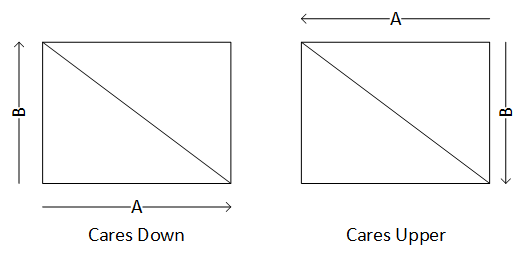
\includegraphics[width=0.6\textwidth]{caranormal}
	\caption{Patró per càlcul de normals en les cares}
	\label{fig-normalcara}
\end{figure}

\begin{figure}[!h]
\centering
  	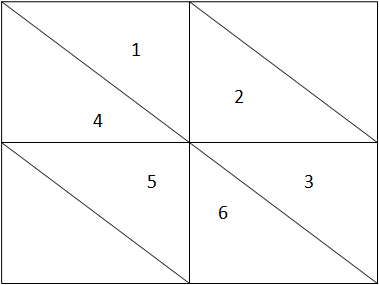
\includegraphics[width=0.4\textwidth]{vertexnormal}
	\caption{Patró per càlcul de normals en un vèrtex}
	\label{fig-normalvertex}
\end{figure}

\newpage
Un cop realitzat el procés de generació l'aplicació haurà generat una malla que podem obrir en qualsevol editor com podem veure en la figura \ref{fig-meshlab}

\begin{figure}[!h]
\centering
  	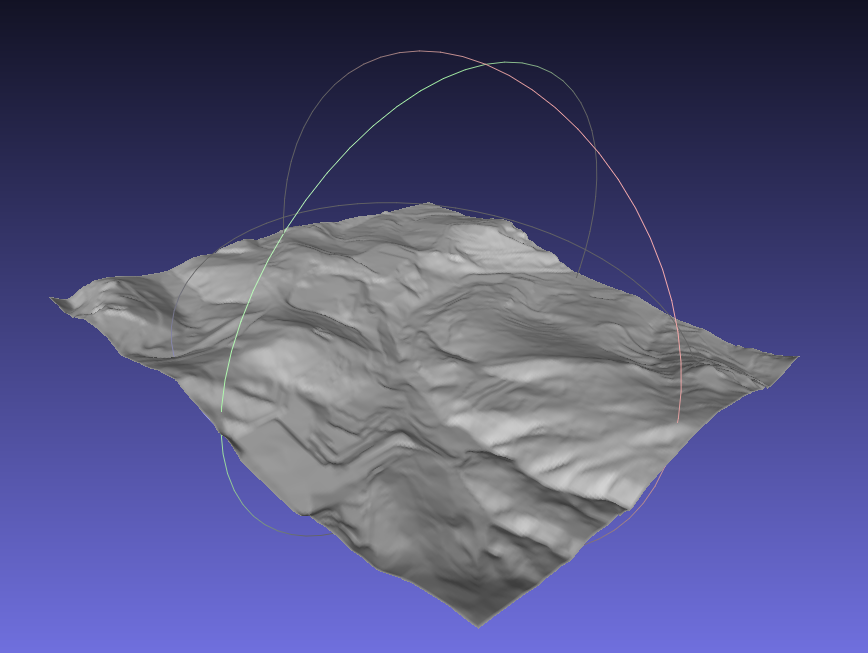
\includegraphics[width=0.45\textwidth]{mesh_example_meshlab}
	\caption{Malla d'un terreny visualitzada en l'aplicació MeshLab}
	\label{fig-meshlab}
\end{figure}

\section{Mòdul: Simulador}

En aquesta secció explicarem els diferents punts dels quals es compon el mòdul de simulació amb el que se cerca l'objectiu de posar a disposició una eina que ens permeti simular un viatge amb un vehicle genèric per sobre d'un terreny obtenint imatges des de diferents càmeres configurades anteriorment.

\subsection{Vehicle i visualització}
Aquesta part serà l'encarregada de donar la interfície per moure un vehicle genèric pel nostre món simulat, aquest vehicle es configurarà amb una sèrie de càmeres (Vegeu més a la secció \ref{section:cameraconfig}) que es podran visualitzar en la pantalla i generar imatges de cada una d'elles. Com es pot veure a la figura \ref{fig-screenshotsimulator} veurem una vista inicial del nostre vehicle des de la part posterior, i estarem veient en un requadre petit de la nostra pantalla la imatge generada per la càmera inferior.

\subsection{Terreny}
El terreny és carregat mitjançant codi obtenint la malla i assignant aquesta a un objecte carregat en el món al qual li canviarem el fitxer textura que utilitzara per tal de renderitzar com és veu el terreny. 
\\
\\
Aquest material tindrà la capacitat de canviar entre diverses textures per tal de poder carregar informació en diferents espectres i canviar aquesta visualització segons un paràmetre que és podrà canviar des de el client Python.

\subsection{Comunicació amb el client d'scripts}

Aquesta comunicació es farà utilitzant el protocol RPC, en aquest cas s'utilitza la llibreria Rpclib\cite{rpclib} per a C++ per la creació del servidor, la gestió del servidor RPC es fa mitjançant una llibreria estàtica escrita en C++ que s'incorpora al projecte d'Unreal per tal d'abstraure la comunicació RPC amb les crides a codi Unreal.

\begin{figure}[!h]
\centering
  	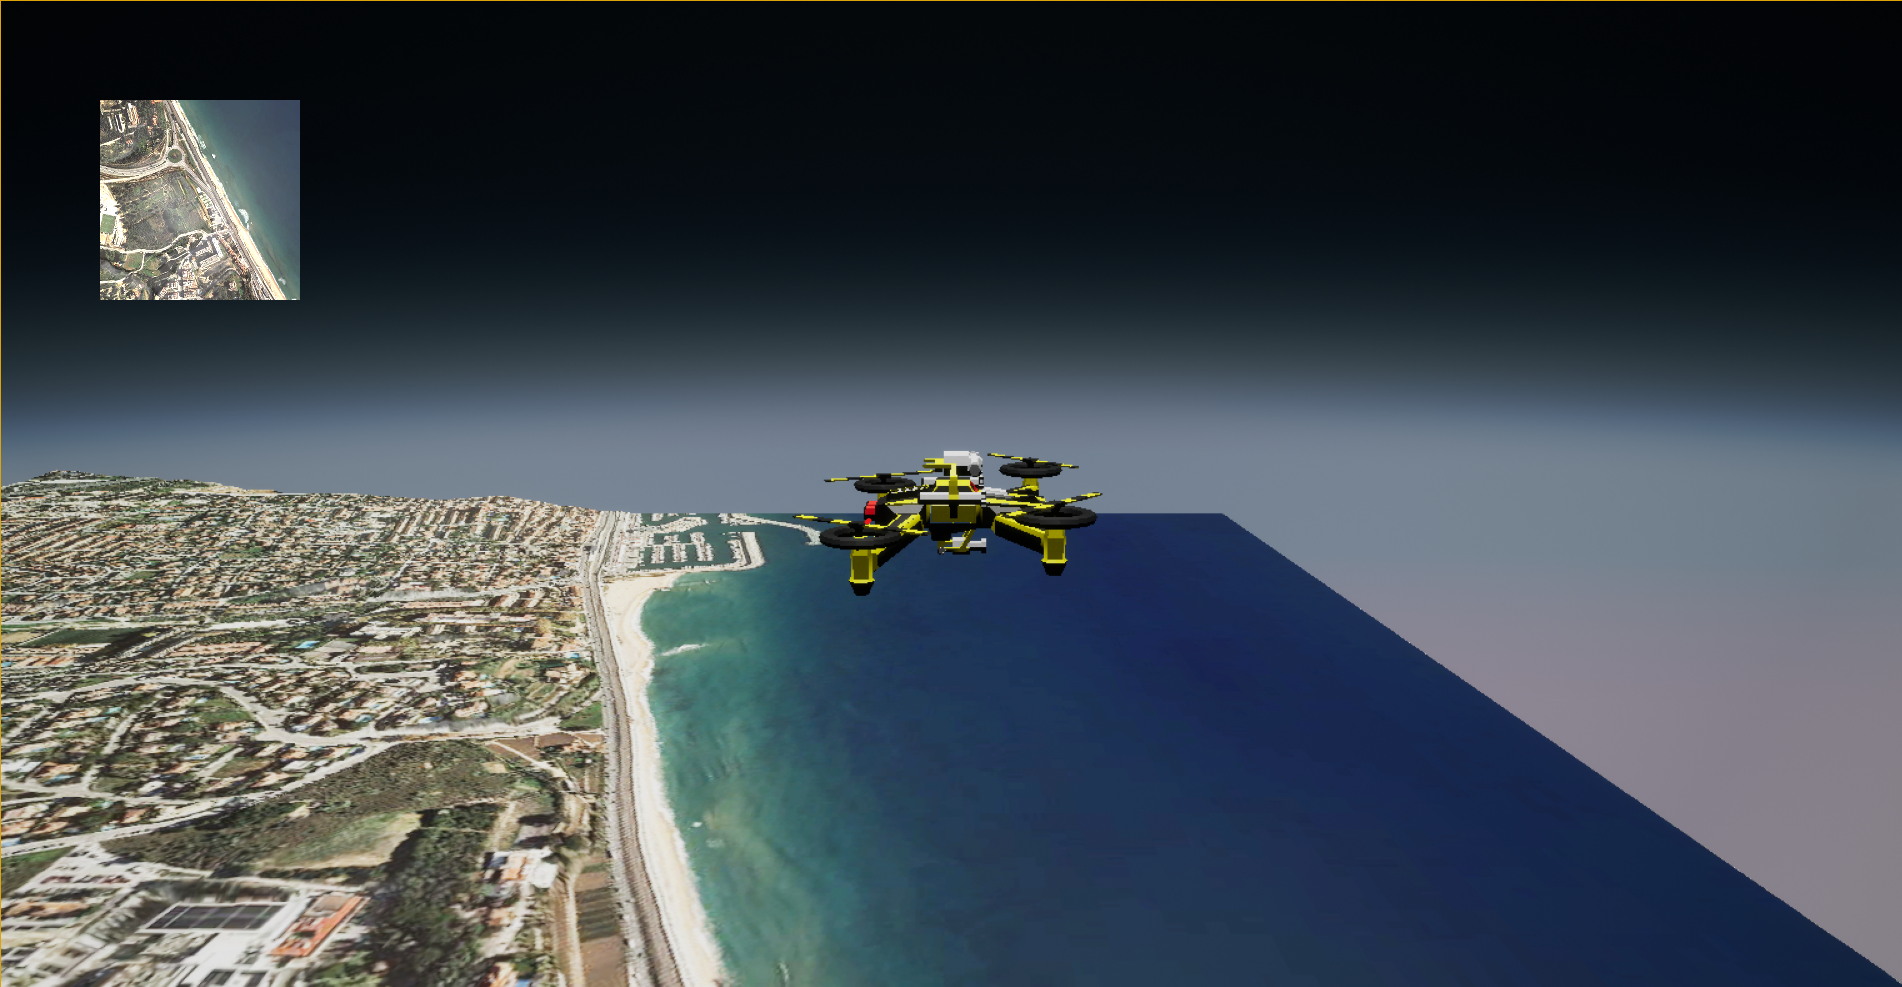
\includegraphics[width=0.7\textwidth]{simulator_example}
	\caption{Captura de pantalla del simulador}
	\label{fig-screenshotsimulator}
\end{figure}

\begin{thebibliography}{11}

\bibitem{ogc}
Open Geospatial Consortium (OGC) -  \url{http://www.opengeospatial.org/} [08/04/2019]

\bibitem{wms}
Web Map Service (WMS) -  \url{https://www.opengeospatial.org/standards/wms} [08/04/2019]

\bibitem{wcs}
Web Coverage Service (WCS) -  \url{https://www.opengeospatial.org/standards/wcs} [08/04/2019]

\bibitem{icgc}
Institut Cartogràfic i Geològic de Catalunya (ICGC) - \url{http://www.icgc.cat/ca/} [08/04/2019]

\bibitem{wavefrontobj}
Wavefront .obj file - \url{https://en.wikipedia.org/wiki/Wavefront_.obj_file} [09/04/2019]

\bibitem{rpclib}
RPC Lib - Modern mgspack-rpc for C++ - \url{http://rpclib.net/} [10/04/2019]


\end{thebibliography}

\newpage
\appendix

\section*{Apèndix}

\setcounter{section}{1}

\subsection{JSON d'exemple per la configuració de GEOTool}
\label{appendix:geotoolconfig}
\lstinputlisting{geotoolconfig.json}

\subsection{Codi per la generació d'una malla 3D a partir d'un fitxer d'altures}
\label{appendix:generateobj}
\lstinputlisting[language=Python]{generateobj.py}


\end{document}

